\documentclass[11pt,twoside,english,singlespacing,headsepline,consistentlayout]{auxiliary/si-msc-thesis}

\usepackage[utf8]{inputenc} % Required for inputting international characters
\usepackage[T1]{fontenc} % Output font encoding for international characters

\usepackage{lipsum}
\usepackage{mathpazo}
\usepackage{setspace}

\usepackage{lipsum}
\usepackage{float}
\usepackage{listings}
\usepackage{wrapfig}
\usepackage{algorithm}
\usepackage{algpseudocode}
\usepackage{subcaption}
\usepackage{graphicx}
\usepackage{csquotes}
\usepackage{lscape}

\usepackage{setspace}

\usepackage{blindtext}
\usepackage{listings}

\usepackage{amsthm, amssymb}

\theoremstyle{definition}
\newtheorem{definition}{Definition}

\renewcommand\lstlistingname{Data}
\renewcommand\lstlistlistingname{Data Sources}

\usepackage{xcolor}
%\usepackage[dvipsnames]{xcolor}
\definecolor{codegreen}{rgb}{0,0.6,0}
\definecolor{codegray}{rgb}{0.5,0.5,0.5}
\definecolor{codepurple}{rgb}{0.57,0.36,0.51}
%\definecolor{backcolour}{rgb}{0.95,0.95,0.96}

\lstdefinestyle{mystyle}{
    %backgroundcolor=\color{backcolour},   
    commentstyle=\color{codegray},
    keywordstyle=\color{codepurple},
    numberstyle=\tiny\color{codegray},
    stringstyle=\color{codegreen},
    basicstyle=\ttfamily\footnotesize,
    breakatwhitespace=false,         
    breaklines=true,                 
    captionpos=b,                    
    keepspaces=true,                 
    %numbers=left,                    
    %numbersep=5pt,                  
    showspaces=false,                
    showstringspaces=false,
    showtabs=false,                  
    tabsize=2,
    xleftmargin=7pt,
}
\lstset{style=mystyle}

\usepackage{parcolumns}

\usepackage{hyperref}
\addto\extrasenglish{
    \def\sectionautorefname{Section}
    \def\subsectionautorefname{Subsection}
}

\usepackage{tikz}

\newcommand\encircle[1]{%
  \tikz[baseline=(X.base)] 
    \node (X) [draw, shape=circle, inner sep=0] {\strut #1};}

\lstdefinelanguage{algebra}
{morekeywords={import,sort,constructors,observers,transformers,axioms,if,
else,end},
sensitive=false,
morecomment=[l]{//s},
}

\newcommand{\quotes}[1]{``#1''}

\usepackage{listings}
\lstloadlanguages{Ruby}



%%%%%%%%%%%%%%%%%%%%%%%%%%%%%%%%%%%%%%%%%%%%%%%%%%%%%%%%%%%%%%%%%
%%%	MARGIN SETTINGS %%%%%%%%%%%%%%%%%%%%%%%%%%%%%%%%%%%%%%%%%%%%%
%%%%%%%%%%%%%%%%%%%%%%%%%%%%%%%%%%%%%%%%%%%%%%%%%%%%%%%%%%%%%%%%%

\geometry{paper=a4paper, inner=2.5cm, outer=2.5cm, bindingoffset=0cm, top=0.2cm, bottom=2cm, head=13.6pt
	%showframe, % Uncomment to show how the type block is set on the page
}


%%%%%%%%%%%%%%%%%%%%%%%%%%%%%%%%%%%%%%%%%%%%%%%%%%%%%%%%%%%%%%%%%
%%%	THESIS INFORMATION %%%%%%%%%%%%%%%%%%%%%%%%%%%%%%%%%%%%%%%%%%
%%%%%%%%%%%%%%%%%%%%%%%%%%%%%%%%%%%%%%%%%%%%%%%%%%%%%%%%%%%%%%%%%
\thesistitle{Evaluating Curriculum Learning in \\ Code Related Tasks} % Your thesis title, this is used in the title and abstract, print it elsewhere with \ttitle
\supervisor{Prof. Rocco \textsc{Oliveto}} % Your supervisor's name, this is used in the title page, print it elsewhere with \supname
\cosupervisor{Prof. Gabriele \textsc{Bavota}}
\examiner{} % Your examiner's name, this is not currently used anywhere in the template, print it elsewhere with \examname
\degree{Masters} % Your degree name, this is used in the title page and abstract, print it elsewhere with \degreename
\author{Carmen \textsc{Armenti}} % Your name, this is used in the title page and abstract, print it elsewhere with \authorname
\addresses{} % Your address, this is not currently used anywhere in the template, print it elsewhere with \addressname

\subject{Computer Science} % Your subject area, this is not currently used anywhere in the template, print it elsewhere with \subjectname
\keywords{} % Keywords for your thesis, this is not currently used anywhere in the template, print it elsewhere with \keywordnames
\university{\href{http://www.university.com}{University of Molise}} % Your university's name and URL, this is used in the title page and abstract, print it elsewhere with \univname
\department{
	\href{http://department.university.com}{Department of Bioscience and Territory}\\
	\vspace{20pt}
    
\includegraphics[scale=0.1]{images/logo.png}\hspace{0.5cm}
    
\includegraphics[scale=0.1]{images/logo-usi.png}
    %
\includegraphics[scale=0.1]{images/logo.png}
    %
\includegraphics[scale=0.3]{images/usilogo.png}
    \vspace{7pt}
} % University/department logo - uncomment to place it} % Your department's name and URL, this is used in the title page and abstract, print it elsewhere with \deptname

\group{\href{http://researchgroup.university.com}{Research Group Name}} % Your research group's name and URL, this is used in the title page, print it elsewhere with \groupname
\faculty{\href{http://faculty.university.com}{Software Security Systems}} % Your faculty's name and URL, this is used in the title page and abstract, print it elsewhere with \facname

\AtBeginDocument{
\hypersetup{pdftitle=\ttitle} % Set the PDF's title to your title
\hypersetup{pdfauthor=\authorname} % Set the PDF's author to your name
\hypersetup{pdfkeywords=\keywordnames} % Set the PDF's keywords to your keywords
}


%\thesistitle{Evaluating \\ Curriculum Learning in \\ Software Engineering tasks}

%comment to not have subtitle
%\thesissubtitle{Master thesis in Software Analytics} 

%\author{Carmen Armenti}

%\monthyear{October 2022}

%\supervisor{Prof. Rocco Oliveto}

% if you need to add or remove co-supervisors go into titlepage.tex and comment correspondingly

%\cosupervisorone{Prof. Gabriele Bavota}
%\cosupervisortwo{}

%%%%%%%%%%%%%%%%%%%%%%%%%%%%%%%%%%%%%%%%%%%%%%%%%%%%%%%%%%%%%%%%%
%%%	FRONT MATTER %%%%%%%%%%%%%%%%%%%%%%%%%%%%%%%%%%%%%%%%%%%%%%%%
%%%%%%%%%%%%%%%%%%%%%%%%%%%%%%%%%%%%%%%%%%%%%%%%%%%%%%%%%%%%%%%%%

\onehalfspacing
%\doublespacing

\begin{document}

\frontmatter
\pagestyle{plain}

%%%%%%%%%%%%%%%%%%%%%%%%%%%%%%%%%%%%%%%%%%%%%%%%%%%%%%%%%%%%%%%%%
%%%	TITLE PAGE %%%%%%%%%%%%%%%%%%%%%%%%%%%%%%%%%%%%%%%%%%%%%%%%%%
%%%%%%%%%%%%%%%%%%%%%%%%%%%%%%%%%%%%%%%%%%%%%%%%%%%%%%%%%%%%%%%%%

%%%%%%%%%%%%%%%%%%%%%%%%%%%%%%%%%%%%%%%%%%%%%%%%%%%%%%%%%%%%%%%%%%
%%%	TITLE PAGE %%%%%%%%%%%%%%%%%%%%%%%%%%%%%%%%%%%%%%%%%%%%%%%%%%
%%%%%%%%%%%%%%%%%%%%%%%%%%%%%%%%%%%%%%%%%%%%%%%%%%%%%%%%%%%%%%%%%

\begin{titlepage}

\hspace{-11.8mm} 
%
\includegraphics[width=65mm]{auxiliary/Grid-System-USI-Software.pdf}

\linespread{1.25}
\vspace{24mm} \hspace{26mm} \parbox{127mm}{{\bf {\huge {\textsc{\ttitle}}}\par}}
\linespread{1}

\ifthenelse{\boolean{@subtitle}}
	{\vspace{4mm} \hspace{26mm} \parbox{127mm}{{\bf {\large {\em {\subtitle}}}}}\vspace{10mm}}
	{\vspace{26.5mm}}

\vspace{16mm} \hspace{26mm} \parbox{127mm}{{\Large {\textbf{\authorname}}}}

\vspace{24mm} \hspace{26mm} {\large \moyear}

\vspace{48mm} \hfill {\large {\em Supervised by}}\\ \vspace{1mm} \hfill {\large {\bf {\supname}}}

\vspace{8mm} \hfill {\large {\em Co-Supervised by}}\\ \vspace{1mm} \hfill {\large {\bf {\cosupnameone}}}

%comment out if it does not apply

%\vspace{1mm} \hfill {\large {\bf {\cosupnametwo}}}

%\vspace{1mm} \hfill {\large {\bf {\cosupnamethree}}}


\vfill

%\hfill \noindent {\textsc{Software \& Data Engineering Master Thesis}}

\end{titlepage}
\begin{titlepage}
    \begin{center}
    
    \vspace*{.01\textheight}
    {\scshape\LARGE \textbf \univname\par} % University name
    {\scshape\LARGE \deptname\par}\vspace{0.5cm} 
    \textsc{\LARGE \textbf{Double Master's Degree}}\\[0.1cm] % Thesis type
    \footnotesize{\textsl{jointly organized by UNIMOL and USI}}\\[0.5cm]
    %\textsl{in}\\[0.3cm]
    {\textsc{in}}\\[0.5cm]
    %\textup{jointly organized by UNIMOL and USI}\\
    %\textup{in}\\[0.3cm]
    \textsc{\LARGE Secure Software and Data Engineering}\\[0.5cm]
    
    \HRule \\[0.1cm] % Horizontal line
    {\huge \bfseries \ttitle\par}\vspace{0.4cm} % Thesis title
    \HRule \\[1.2cm] % Horizontal line
     
    \begin{minipage}[t]{0.4\textwidth}
    \begin{flushleft} \large
    \emph{Author:}\\
    \authorname
    %\href{http://www.johnsmith.com}{\authorname} % Author name - remove the \href bracket to remove the link
    \end{flushleft}
    \end{minipage}
    \begin{minipage}[t]{0.4\textwidth}
    \begin{flushright} \large
    \emph{Supervisor:} \\
    \href{https://dibt.unimol.it/staff/oliveto/}{\supname}\\[0.5cm] % Supervisor name - remove the \href bracket to remove the link 
    \emph{{Co-supervisor:}} \\
    \href{https://www.inf.usi.ch/faculty/bavota/#}{\cosupname}\\[0.5cm]
    \end{flushright}
    \end{minipage}\\[2cm]
     
    \vfill
    
    %\large \textit{A thesis submitted in fulfillment of the requirements\\ for the degree of \degreename}\\[0.3cm] % University requirement text
    %\textit{in the}\\[0.4cm]
    %\groupname\\\deptname\\[2cm] % Research group name and department name
    
    \vfill
    
    %{\large Software Analytics}\\
    %{\large October 27, 2022}\\[0.9cm]

    {\footnotesize{\textsl{The double degree programme involves the Master's degree programme “Software System Security” (M.Sc.) \\ 
    at UNIMOL and “Software and Data Engineering” (M.Sc.) at USI.}}}\\[0.9cm]
    
    %{\large \today}\\[4cm] % Date

    {\large Software Analytics}\\[0.1cm]
    {\large October 27, 2022}
    
    \vfill
    \end{center}
\end{titlepage}



%----------------------------------------------------------------------------------------
%	QUOTATION PAGE
%----------------------------------------------------------------------------------------
\cleardoublepage
\vspace*{0.2\textheight}

\begin{flushright}
	%\noindent\enquote{\itshape Everything is just a function of the amount of time put into it.}\bigbreak
	\noindent\enquote{\itshape Everything is just a function of the amount of time put into it.}\bigbreak
\end{flushright}
    

%%%%%%%%%%%%%%%%%%%%%%%%%%%%%%%%%%%%%%%%%%%%%%%%%%%%%%%%%%%%%%%%%
%%%	ABSTRACT %%%%%%%%%%%%%%%%%%%%%%%%%%%%%%%%%%%%%%%%%%%%%%%%%%%%
%%%%%%%%%%%%%%%%%%%%%%%%%%%%%%%%%%%%%%%%%%%%%%%%%%%%%%%%%%%%%%%%%

%\input{Abstract}

%%%%%%%%%%%%%%%%%%%%%%%%%%%%%%%%%%%%%%%%%%%%%%%%%%%%%%%%%%%%%%%%%
%%%	DEDICATION & ACKNOWLEDGEMENTS %%%%%%%%%%%%%%%%%%%%%%%%%%%%%%%
%%%%%%%%%%%%%%%%%%%%%%%%%%%%%%%%%%%%%%%%%%%%%%%%%%%%%%%%%%%%%%%%%

%\input{ded-acks}

%%%%%%%%%%%%%%%%%%%%%%%%%%%%%%%%%%%%%%%%%%%%%%%%%%%%%%%%%%%%%%%%%
%%%	PREAMBLE %%%%%%%%%%%%%%%%%%%%%%%%%%%%%%%%%%%%%%%%%%%%%%%%%%%%
%%%%%%%%%%%%%%%%%%%%%%%%%%%%%%%%%%%%%%%%%%%%%%%%%%%%%%%%%%%%%%%%%

\tableofcontents 
\listoffigures 
\listoftables

%----------------------------------------------------------------------------------------
%	DEDICATION
%----------------------------------------------------------------------------------------
\vspace*{.03\textheight}
\begin{flushright}
	\dedicatory{To my family, \linebreak without whom I would not be who I am.} 
\end{flushright}

%%%%%%%%%%%%%%%%%%%%%%%%%%%%%%%%%%%%%%%%%%%%%%%%%%%%%%%%%%%%%%%%%
%%%	MAIN MATTER %%%%%%%%%%%%%%%%%%%%%%%%%%%%%%%%%%%%%%%%%%%%%%%%%
%%%%%%%%%%%%%%%%%%%%%%%%%%%%%%%%%%%%%%%%%%%%%%%%%%%%%%%%%%%%%%%%%

\mainmatter
 
\pagestyle{thesis} 

 \chapter{Introduction}
Humans and animals acquire an extensive and flexible repertoire of complex behaviors through learning. They can perform
much more complex tasks that they can acquire using simple trial and error learning. 
This gap is filled by teaching indeed, and in education contexts one important method is \textit{shaping}. Shaping starts with a task analysis in which a desired
behavior is broken down into smaller and more manageable steps that would move the learner, namely the child, successively closer to that desired behavior. Once the small approximations of the desired behavior are clearly
identified, one must select the reinforcement to be used and make sure that everyone working with the tutee knows which behavior, when, and how to reinforce the approximations.
Data on the behavior should be collected and reviewed by the team. The program must continue until the learner demonstrate the desired behavior.
In order for shaping to be successful, it is important to clearly define the behavioral objective and the target behavior. Also, in order to gradually achieve the target, 
a teacher must know when to deliver or withhold reinforcement. \\
The term \textit{shaping} was first coined 
by B. F. Skinner\footnote{Skinner is an american psychologist, behaviorist, author, inventor, and social philosopher.}, 
who described it as a \textsl{"method of successive approximations"}. In shaping indeed, a sequence of intermediate, simple tasks is taught, in order to aid acquisition of an original,
complex task. Practically shaping shares the same idea of the divide-and-conquer concept.\\
Even though all the previous said looks to be more appropriate
to behavioral engineering\footnote{Behavioral engineering, also called Applied behavioral analysis (ABA) is a scientific discipline that applies
empirical approaches based upon the principles of respondend and operant conditioning to change behavior of social significance.}
- being it related to the attempts that experts of the field put into practice to change human or animal behaviors - 
shaping has also been related to machine and deep learning.\\

\section{Application Context}
Bengio \textit{et al.} \cite{bengio2009curriculum} in their work \textsl{"Curriculum Learning"} are the first to relate the shaping concept
to the context of machine learning theory, calling the training strategy of organizing the training in a meaningful order \textit{curriculum learning} indeed.
Curriculum learning was originally inspired by the learning experience of humans, since human beings tend to learn better and faster when 
they are first introduced to simpler concepts and exploit previously learned concepts and skills to ease the learning of new abstractions.
However, the basic idea of training a learning machine with a curriculum method can be traced back
at the very least to Elman \cite{ELMAN199371}. Elman realized a concept described in terms of \textit{less is more}, in the context of the learning 
of grammars in simple recurrent networks. The idea was to use an initial phase of training with only the simplest rules of the grammar.
The experimental results, based on learning a simple grammar with a recurrent network, suggested that
successful learning of grammatical structure depends, rather than on innate knowledge of grammar,
on starting with a limited architecture that is at first quite restricted in complexity, but afterward expands its resources
gradually as it learns. Such conclusions are important for developmental psychology, because they 
illustrate the adaptive value of starting, as human infants do, with a simpler initial state, and then building on that to develop
more and more sophisticated representations of structure. The question of guiding learning of a recurrent neural network for learning
a simple language and increasing its capacity along the way was revisited by Krueger \& Dayan \cite{krueger2009},
who used an unelaborated form of the 
long short term memory (LSTM) model, studying
the additional role that shaping might play in generating complex behavior in tasks, and providing
evidence for faster convergence using a shaping-like procedure. Similar ideas were also explored
in robotics, where reinforcement learning was applied by gradually making the learning task more difficult.

\section{Motivations and Objectives}
\label{chapter:MAO}
Whether machine learning algorithms benefit from a similar training strategy is a question that has been widely answered so far, 
every time differently, depending on the task experimented and on the results aimed. Without surprise, \textit{curriculum learning}
has been found most helpful in end-to-end neural network architectures \cite{bengio2009curriculum},
given that the performance that an artificial network can achieve mostly depends on the quality of training data given to it.\\
Recently, the application of \textit{curriculum learning} is also studied for Neural Machine Translation (NMT), that translates text from a source
language to a target language in an end-to-end fashion with a single neural network. On top of that, the performance of 
NMT has been improved significantly in recent years, as these architectures evolved from the initial Recurrent Neural Network (RNN) based models, to convolutional
seq2seq models and further to Transformer models. \\
\newline
Since many clarified when and why a \textit{curriculum} or \textit{starting small} strategy can be of benefit
to machine learning algorithms, and given that none of the previous work in the current state of the art 
involved software engineering tasks, we decided to bridge this gap focusing our attention on 3 software engineering tasks: \textbf{bug-fixing}, 
\textbf{code summarization}, and \textbf{log generation}.\\
\newline
Not only are curriculum learning applications of benefit to \textit{improving model performances
on target tasks} - given by the metaphor with 
the effective human-based learning approach, but also of \textit{accelerating the training process}.
However, since we worked with a NMT and given that training a NMT model is a time-consuming task a priori, 
we were curious to see results in terms of both the two most significant requirements 
aforementioned. 

%in major machine learning research

\section{Results}
By and large, the CL training times for the bug-fixing 
and code summarization tasks were not that much different from
the plain-training process times without curricula; quite the opposite, as for the log generation task, CL training took slightly longer.\\
In terms of performances, bug-fixing task is the only one who showed a significant improvement; code summarization and log generation 
task experiments instead reported quite similar results, as for the comparison between plain and curriculum training.
However, it is necessary saying that if as to the bug-fixing task the neural architecture was the one 
used to originally test and evaluate such task in \cite{Tufano2019}, as regards to the other two tasks 
the curriculum approach was tested on the very same NMT framework - instead of being 
tested on the neural networks used in the original pieces of work \cite{Leclair2020}, \cite{Mastropaolo2022}.

\section{Document Structure}
This thesis is organized as follows:
\begin{itemize}
    \item Chapter 2 - Deep Learning and Curriculum Learning: related works in the current state of the art;
    \item Chapter 3 - Deep Learning Applications to Software Engineering Tasks: theoretical background and other works;
    \item Chapter 4 - Evaluating CL in Software Engineering Tasks: definition and development of CL approach considered;
    \item Chapter 5 - Analysis of results: assessment for each of the task of the CL approach used;
    \item Chapter 6 - Conclusion and Future Works: summary and possible future developments.
\end{itemize}

 \chapter{Deep Learning and Curriculum Learning}
Humans are different from other species in many ways, but two of them are particularly noteworthy. 
First of all, humans display an exceptional capacity to learn;
moreover, humans are remarkable for the long time they take to reach maturity. Human beings need about two decades to be trained as fully functional adults for our society and it may
be argued that, through culture, learning has created the basis for a non-genetically based transmission of behaviors and habits which might
accelerate the evolution of our species. Infancy and childhood are times of great vulnerability for the young, when the first skills are developed and when the adults who
must care for and protect their own young go through a severe restriction of their range of activities. Then, why would evolutionary process not prune a long period of 
immaturity from our species? Previous research carried out by Elman \textit{et al} \cite{ELMAN199371} at the intersection of cognitive science
and machine learning underline that it is important to remember that the evolution looks at the whole individuals rather than at the value of isolated traits; the adaptive success of individuals therefore is 
determined by the joint interaction of all their traits. Thus, it might be that to understand the persistence of one trait with apparently negative consequences - such as the lenghty period of immaturity, possible interactions
with other traits - such as the ability to learn - may need to be considered. The perfect example of such an interaction, is that in human beings the greatest learning occurs precisely in the period of time
when they are undergoing major changes, during childhood indeed.\\

\section{State of the art}
In humans, learning and development interact in a way as important as non-obvious; maturational changes might provide the enabling 
conditions which allow learning to be most effective. It is a matter of fact that humans need about two decades to be trained as fully functional 
adults, and the higher the training is organized, the better the knowledge of the person. Humans in fact learn much better when the examples are not randomly presented, but organized in such a way 
where the amount of concepts is incremented gradually, and where the complexity of them increases over time. The majority of education systems are organized in order to illustrate 
different concepts at different times, exploiting previously learned notions to ease the learning of new abstractions. By choosing which examples to present and in which order to explain them to the learning system, one can guide
training and consequently increase the speed at which learning can happen. This is the same idea exploited in \textit{animal training} by psychologists Skinner (1958), Peterson (2004) and Krueger \& Dayan (2009)
where it is called \textit{shaping}. \\
In the context of machine learning, such a meaningful learning process is known as \textit{curriculum learning}, whose basic idea - traced back to Elman - is to start small, learn easier aspects
of the task, and then gradually increase the difficulty level.
Inspired by human learning in fact, curriculum learning (CL) is a training strategy that emphasizes
the order of training instances in a computational learning setup.
As a feature of human learning, curriculum - or even better learning in a meaningful way -
has been transferred to machine learning, thus creating the subdiscipline named
\textit{curriculum learning}.
Essentially, human education is organized as curricula, by starting small indeed, and gradually presenting more complex
concepts. The paramount hypothesis is that simpler instances should be learned
during the first steps as building blocks, to then learn more complex ones. Several experiments on sentiment 
analysis task and tasks similar to sequence prediction tasks in NLP carried on by Cirick \textit{et al} \cite{Cirik2016VisualizingAU} prove that
curriculum learning has positive effects on LSTM's internal states, by biasing the model through building constructive representations. 
Specifically, the internal representation at the previous timestep is used as building block for the next one, thus
contributing at the final prediction.

In traditional machine learning algorithms all the training examples are randomly presented to the model,
thus ignoring the different complexities of data instances and the learning status of the current model. 
Owning to this, it is fairily intuitive wondering if the curriculum training strategy could ever benefit machine learning.
Extensive experiments from early \cite{bengio2009curriculum}, \cite{kumar2010self}, \cite{zaremba2014learning} to recent works \cite{fan2018learning}, \cite{graves2017automated}, \cite{hacohen2019power}, \cite{platanios2019competence} in various applications of machine learning show that such strategy is of benefit to this field, but not always, and 
because of that the power of introducing the curriculum-like strategy depends on how the curriculum for specific applications and datasets is designed.

\section{Curriculum Learning related works}
As the idea of CL provide a general training strategy beyond specific machine learning
tasks, its power have been exploited in considerably wide application scopes, including supervised learning
tasks within computer vision, natural language processing (NLP), healthcare prediction, various
reinforcement learning (RL) tasks, as well as other applications such
as graph learning, and neural architecture search (NAS). As already mentioned in \ref{chapter:MAO}, the advantages of applying CL
training strategies to miscellaneous real-world scenarios can be mainly summarized as (i) improving the model perfomrance on 
target tasks, and (ii) accelerating the training process, which cover the two most significant 
requirements in most of the machine learning research. 
To provide an illustration,
Platanios \textit{et al.} \cite{platanios2019competence} present 
a personal framework that consists of a way of deciding which training instances
are shown to the model ad different times during training, based on 
an estimated difficulty of a sample and on the current competence
of the model. Thus, filtering training samples prevents the model from 
getting stuck in bad local optima, making it converge faster and reach
a better solution than the common approach of uniformly 
sampling training examples. Their experiment shows that CL helps the 
neural machine translation model reduce training time by up to 70\%, whie at the 
same time obtaining accuracy improvements of up to 2.2 BLEU points, compared
to plain training without any curricula. In \cite{florensa2017reverse} Florensa 
\textit{et al.} talk about curriculum learning as a reverse curriculum technique. 
They propose a method to learn goal-oriented tasks without requiring
any prior knowledge, other than obtaining a single state in which
the task is achieved. They dimonstrate that their approach is 
based on a reverse training, where the robot gradually learns to reach 
the goal from a set of start states increasingly far from the goal.
That approach resulted in solving hard problems, not solvable 
by state-of-the-art reinforcement learning methods.

\section{Curriculum Learning application in Deep Learning tasks}
Training neural networks is traditionally done by providing a sequence of 
random mini-batches sampled uniformly from the entire training data. Conversely, curriculum learning
involves the non-uniform sampling of mini batches, on the training of deep networks.
However, understanding why and when \textit{starting small} strategies can 
benefit machine learning algorithms is a question that every scholar try to contribute to.
Bengio \textit{et al.} \cite{bengio2009curriculum} other than showing several cases where very simple
multi-stage curriculum strategies give rise to improved generalization and faster convergence, 
contribute to the question introducing a hypothesis which might help to explain 
some of the advantages of a curriculum strategy. They argue that a well chosen curriculum 
strategy can act as a continuation method. Intuitively, continuation methods are optimization
strategies for non-convex criteria which first optimize a smoother and easier version of the problem to 
reveal the "global picture", and then gradually consider less smoothing versions, until the tarhet objective of 
interest. Therefore, continuation methods provide a sequence of optimization objectives, starting with an objective for which
it is easy to find a global minimum, and tracking the local minima throughout the training. In this way, continuation methods
guide the training towards better regions  and the local minima learned from easier objectives have better
generalization ability and are more likely to approximate global minima.
To test this hypothesis, they turn the attention to training of deep
architectures, which have been shown to involve good solutions in local minima that are almost impossible to find 
by \textit{random initialization}. Generally, deep learning methods try 
to learn feature hierarchies, i.e., features at higher levels are formed by the composition of lower level features.
As a consequence, automatically learning multiple levels of abstracion may allow a system to induce complex functions mapping the input to the 
output directly from data, without depending heavily on human-crafted features.
One possible theoretical motivation for deep architectures comes from complexity theory. Some functions, in fact, can 
be represented with an architecture of depth \textit{k} but require an exponential size architecture when the depth 
is restricted to be less than \textit{k}. Training deep networks, however, involves a potentially 
intractable non-convex optimization problem \cite{bengio2009curriculum}. There were no good algorithms for training 
fully-connected deep architectures before 2006, when Hinton introduced a learning algorithm that greedily trains one layer at a time, exploiting an unsupervised
generative learning algorithm for each layer. It is conceivable that by training 
each layer one after the other, the network is organized in such a way that it can first learn the simpler
concepts, represented in the first layer indeed, then sligthly more abstract ones, represented in the second layer, and so on.
Not long after, strategies for building deep architectures from related variants were proposed %add ref 
and these works showed the advantage of those frameworks over shallow ones, and of the unsupervised 
pre-training strategy in a variety of settings.\\

\section{Definition of Curriculum Learning}
Based on all the previous works in the first place provided in behavior and 
cognitive science literature, the concept of CL was first proposed in \cite{bengio2009curriculum} with 
experiments on supervised visual and language learning tasks, exploring when and why curriculum could benefit machine learning.
The original definition of CL refers to a curriculum as a sequence of training criteria 
over \(T\) training steps \( C = \left \langle Q_1, ..., Q_t, ..., Q_T \right \rangle\), where each  
criterion \(Q_t\) is a reweighting of the target training distribution \(P(z)\): \(Q_t(z) \propto W_t(z)P(z)\), for 
each instance in the training set. In the definition the following three conditions were considered:
\begin{itemize}
    \item the entropy of distributions gradually increases, \(H(Q_t) < H(Q_{t+1})\);
    \item the weight for any example increases, \(W_t(z) \leq W_{t+1}(z) \forall z \in D\);
    \item \(Q_T(z) = P(z)\).
\end{itemize}
So, curriculum learning is the training strategy that trains a machine learning model
with a curriculum. The first of the above conditions means that the diversity 
and the information of the training set should gradually increase. More specifically,
the reweighting of examples in later steps increases the probability of sampling slightly more difficult examples.
The second condition instead means to gradually add more training examples, letting the size of the training set increase. 
Finally, the last condition
means that the reweighting of all examples is uniform and the training is carried on the target training set.\\
At a more abstract level, a curriculum can be seen as a sequence of instance selection or example reweighting along the training process in order to achieve faster convergence or better generalization, 
which is beyond the "easy to hard" or "starting small" principles. 

\section{A general CL framework}
In a nutshell, curriculum learning means "training from easier data to harder data" \cite{Wang2020}. More specifically the
core idea is to "start small" \cite{ELMAN199371}, train the machine learning model with easier subtasks, to then gradually increase
the difficulty level of subtasks until the whole training dataset is used.\\
Bearing in mind the strategy of training from easier to harder data, to design such a curriculum idea 
(i), what kind of training data is supposed to be easier than other data, (ii) and when is appropriate to present more harder
data for training - and how much more - must necessarily be decided.
Technically, those 2 issues can be abstracted in the concepts of a Difficulty Measurer, that decides the "easiness"
of each data instance to start the training process from, and a Training Scheduler, that rules the sequence of data subsets during 
the whole training process \cite{Wang2020}.
Therefore, Difficulty Measurer together with Training Scheduler constitute a general framework for curriculum design,
as illustrated in Figure ~\ref{fig:CLdesign}.
\begin{figure}[h]
    \begin{center}
        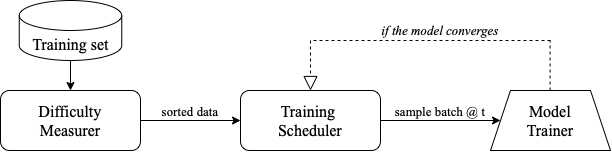
\includegraphics[width=0.55\textwidth]{/Users/carmenarmenti/Desktop/Thesis document/images/predefinedCL.png}
        \caption{\label{fig:CLdesign}Predefined Curriculum Design.}
    \end{center}
\end{figure}
First of all, the Difficulty Measurer sorts all the training examples from the easiest 
to the hardest and passes them to the Training Scheduler. Then, at each training epoch \textit{t}, the Training Scheduler
samples a batch of training instances from the easier subset and gives them to the Model Trainer for training.\\
As training epochs increase, the Scheduler decide when to sample from more harder data, generally until uniform sampling
from the whole training set. This schedule either depends on the training loss feedback from the Model Trainer, or on some other
parameters that implies that the model would deverge, if left to training for more epochs.\\
Moreover, a distinction between \textbf{predefined CL} and \textbf{automatic CL} must be clarified. The first refers to the framework
where both the Difficulty Measurer and Training Scheduler are defined by human prior knowledge, thus with no data-driven
algorithms involved; the latter instead, if any - or both - of the components are designed by data-driven algorithms.\\
Usually, the power of introducting Curriculum into Machine Learning depends on how the curriculum for specific
applications and dataset is designed. Due to this, Difficulty Measurers often relies on the data
characteristics of specific tasks, and most of them are defined by complexity, diversity, or noise estimation
definitions.\\

%%%%%%%%%%%%%%%%%%%%
% NOTES
% As mentioned previously, this is the first work studying LSTM networks
% on software engineering tasks with curriculum learning to our knowledge.

%%%%%%%%%%%%%%%%%%%%

 \chapter{Deep Learning Applications to Software Engineering tasks}
The advent of deep learning (DL) has fundamentally changed the landscape of modern software and in order to cope with 
the increasing complexity of digital system programming, deep learning techniques have recently been proposed 
to enhance software deployment by analysing source code for different purposes, ranging from performance improvement 
to debugging and security assessment. Driven by the success of deep learning in data mining and pattern 
recognition, recent years witnessed an increasing trend for researchers to integrate deep learning with software engineering (SE) 
tasks. In the most typical SE tasks, deep learning helps to generate or summarize source code, predict defects in software, extract requirements from natural language text, 
and many more tasks.
Generally, a DL system is made of several interconnected computational atomic units that form \textit{layers}
which perform mathematical transformations, according to sets of learnable parameters, on input data. These architectures
can be trained for specific tasks updating the parameters according to model configuration on a specific set of training data. \\ Over the years, 
deep learning has developed advancements in many complex tasks often associated with artificial intelligence, within software engineering 
is now comprehended. DL is intertwined with SE, in fact, DL techniques allow to automate or improve existing software 
development tasks nowadays. 

\section{State of the art}
Given the effectiveness by which DL systems are able to learn representations from large data corpora, there is 
ample opportunity to leverage DL techniques to help automate or improve a wide range of code related tasks. 
Software engineering research investigates questions related to the design, development, maintenance, testing and evolution 
of software systems. Previously, the software engineering community has applied traditional machine learning 
techniques to identify interesting patterns and unque relationships within the data to automate or enhance many tasks typically 
performed by developers. Due to recent improvements in computational power and the amount of memory available 
in modern computer architectures, the rise of deep learning has led to a new class of learning algorithms suited for large datasets.
Deep learning represents a fundamental shift in the nammer by which machines learn patterns from data by automatically extracting salient features
for a given computational task, as opposed to relyig upon human intuition. Given the immense amount of data in software repositories that 
can serve as training data, deep learning techniques have ushered in advancements across a range of tasks in software engineering research, including
automatic software fising, code suggestion, defect prediction, feature location among many others. This field of research shows clear potential for
transforming the manner by which a variety of specific software development task are performed.

\section{Software Engineering related works}
Between 2013 and 2015, machine learning techniques were explored on high-level code, starting from a manual 
definition of features to the first deep learning applicactions capable of extracting features from code on their own.
The techniques used are strongly inspired by the background of natural language processing 
- being \textit{most software natural} \cite{hindle2016naturalness} since it is created by human beings - and include n-grams, decision threes, 
and recurrent neural networks (RNN). RNNs in particular have been extensively tested to assess their effectiveness
Rayachev \textit{et al.} \cite{raychev2014code} proposed a code completion strategy that compares n-gram model and recurrent neural networks. 
They implement a technique that firs extract sequences of API calls from the dataset, then apply n-gram to these sequences, and finally use the RNN 
to take the last word in the sequence as input and uses one-hot-encoding to predict probabilies for the most likely next word.
They argue that the n-gram technique can discover regularities between the last \textit{n} - 1 elements of fucntion-calls sequences, whereas RNN can discover
relations at longer distances.


\subsection{Bug fixing task}
Each instance of the dataset is a pair $(m_b, m_f)$, where $m_b$ is a buggy code component and $m_f$ is the
corresponding fixed code. These BFPs were used to train the NMT model, allowing it to learn the translation
from the buggy to the fixed method, thus being able to generate fixing patches.
\subsection{Code summarization task}
Automatic source code summarization is the task of generating short natural language description 
for source code \cite{Leclair2020}. The idea is that a brief description allows programmers to understand
what a chunk of code does and what is the purpose of the program by and large, without necessarily read the code 
itself.\\
%\subsection{Log generation task}
 \chapter{Evaluating Curriculum Learning in Software Engineering tasks}


We adopted the most popular discrete scheduler, known as \textit{Baby Step}, where the complexity of the training
data needs to be gradually increasing. Due to this, a reliable metric to split the initial dataset of each task needed to be defined.
This approach distributes the sorted data into buckets, from easy to hard according to the metric, and starts training with the easiest bucket. 
Starting from the easiest bucket, after a fixed number of training epochs or convergence, the subsequent bucket is merged
into the current training subset - main characteristic of \textit{Baby Step} approach.
Finally, once all the buckets are merged and used, the
training process either stops or continues several extra epochs.\\
Note that, at each epoch the scheduler shuffles the current bucket and samples mini-batches for training.\\

However, before testing curriculum learning approach, we thougth it was strictly necessary reproducing - in the case 
of bug-fixing task - or conducting -  within the framework of the other 2 tasks - the experiment on the modelbase.\\
We worked with a neural network whose configuration is composed by 1-layer bidirectional Encoder, 2-layer Attention 
Decoder both with 256 units, embedding size of 512, and LSTM RNN cells.\\

In this chapter, we present how we applied Curriculum Learning to some of Software
Engineering tasks, i.e. \textit{bug-fixing}, \textit{code summarization}, and \textit{log generation}
tasks. \\
For each of the tasks considered, the following aspects are described thoroughly:
\begin{itemize}
    \item \textbf{Difficulty Measurer}: a measure to sort the datasets' instances is needed, each task was experimented with a different metric; 
    \item \textbf{Training Scheduler}: sequence of data subsets are presented to the model following a training schedule.
\end{itemize}

%\item \textbf{Dataset characteristics}: the datasets used are composed by a couple, where the first element is the source of the training, while the second is the target;

The goal of this study is to asses whether Neural Machine Translation, combined with the Curriculum Learning approach, 
can be used for the tasks experimented. In the following section, the design of our study is described in detail.

% ADDITIONS
% need to add information about training on baseline, i.e. in the introduction you must explain that before trying
% to test the CL approach 

\section{Neural Machine Translation}
The experimented models are based on an Recurrent Neural Network (RNN) Encoder-Decoder
architecture with attention mechanism, frequently used in Neural Machine Translation. This kind of model is composed by two
dominant components:

\begin{itemize}
    \item a RNN Encoder, which encodes a sequence of terms \textbf{x} into a vector representation;
    \item a RNN Decoder, which decodes the vector representation into another sequence of terms \textbf{y}.
\end{itemize}

The model learning is based on a conditional distribution, where the output sequence of terms is conditioned
by the input sequence: \(P(y_1,...,y_m|x_1,...,x_n)\), where \(m\) and \(n\) not necessarly have to have the same length.
The Encoder takes as input a sequence \textbf{x}\(= (x_1,...,x_n)\) and produces
a sequence of states \textbf{h}\(= (h_1,...,h_n)\). The framework relies on a bi-directional
RNN Encoder, which is composed by a backward and a forward RNN, where both are able to create representations taking into account
past and future inputs. Specifically, each state \(h_i\) is the concatenation of the states produced by 
the two RNNs when reading the sequence not only in a forward but also in a backward manner.\\
The RNN Decoder computes the probability of a target sequence \textbf{y}\(= (y_1,...,y_n)\) given \textbf{h}. The probability
of each output term \(h_i\) is computed based on:
\begin{itemize}
    \item the recurrent state \(s_i\) in the Decoder;
    \item the previous \(i - 1\) terms \((y_1,...,y_i-1)\);
    \item a context vector \(c_i\), which constitutes the attention mechanism.
\end{itemize}
The vector \(c_i\) is a weighted average of the states in \textbf{h}, where the weights associated 
to each state allow the model to pay more attention to some parts of the input sequence than to others:
\[c_i = \sum_{t=1}^n a_{it} h_t\]
Precisely, the weigth \(a_{it}\) defines how much the model should take into consideration the term of the sequence in input \(x_i\)
when predicting the target term \(y_t\). Encoder and Decoder are simultaneously trained - instead of sequentially - by minimizing
the negative log likelihood of the target terms, using stochastic gradient descent.
The configuration used by the neural network is composed by 1-layer bidirectional Encoder, 
2-layer Attention Decoder both with 256 units, embedding size of 512, 
and LSTM RNN cells. Bucketing and padding was used to deal with the variable length of the sequences.


\section{Canonical Training}
Before experiment the curriculum learning approach, we reproduced the baseline approaches for each task experimented
that include the conventional technique of randomly ordering the training samples with the aim to investigate how the performance 
of the original models are, compared to the experiment affected by curriculum learning.
\subsection{Bug-fixing}
As for the bug-fixing task, the datasets used to train the NMT model is the union between \textit{small} and \textit{medium} method-level datasets
used by Tufano \textit{et al.} \cite{Tufano2019}. So, we worked with the standard training, evaluation and test set splits of respectively
99.044, 12.381, and 12.380 instances.\\
It is vital to use new data when evaluating a model to prevent the likelihood of overfitting to the 
training set. However, we decided to evaluate our model as we were building it to find the best parameters of 
a model. To evaluate the model while still building and tuning the model, we used the evaluation set. The neural network
was set up to evaluate the model every 1.000 steps. The training was performed for 60k steps as upper bound, 
out of which we considered the best model, early stopping the model before overfitting considering the loss values computed every 1.000 steps.
The best model configuration was then used to run the inference.
Indeed, after the model was trained, it was evaluated on the test set of unseen buggy code. 
Instead of using the classic greeding decoding that selects the output term \(y_i\) with the highest probability, however, we used another decoding
strategy known as Beam Search. 
%[references 2.3.3 michele tufano]. 
The key idea is that the decoding process keeps track of \textit{k}
hypotheses - being \textit{k} the beam size or width.\\
The beam search algorithm selects multiple tokens for a position in a given sequence based on conditional probability. Moreover, the algorithm
can take any number of \textit{N} best alternatives through a hyperparameter known as beam size or width indeed. Conversely to what greedy search does, 
Beam search broad the search to include other words that might fit better apart from the best word for each position in the sequence.
If Greedy search looks at each position in the output sequence in isolation, deciding the word based on highest probability and then moving down to the resto of the sentence,
Beam search also takes the N best output sequences and look at the current preceding words and probabilities compared to the current position that is being decoded in the sequence.\\
We considered the following sizes: 1 - that corresponds to the Greedy Naïve Approach -, 5, 10, 15, 20, 25, 30, 35, 40, 45, 50.

\subsection{Code summarization}
Regarding the task of code summarization, we selected a random sample of 200k instances from a dataset of 2.1 million items.
Also here we considered the canonical division between training, test and evaluation of respectively 200.000, 105.832, and 106.153 instances.
We trained the model on the training set for 20 epochs, that corresponds to 125.000 steps, and we took the best model over the 20 model configuration evaluated after every epoch,
thus using the best checkpoint to run the inference step. This time, to guide the selection of the best configuration, we used the BLEU values computed on the validation set instead of using
the loss function. Conversely, the results are computed on the test set. Indeed, the same way it was done for the previous task, after the training step the model is
evaluated over the test set of unseen functions to generate code summarizations of such methods.\\
The scope of the training here 
was to make the model able to learn how to summarize pieces of code, starting from a sequence of tokenized methods.

%\subsection{Log generation}
%As well as happened in both the previous task experimented, also in log generation we considered the well-known split between training set, test set, and evaluation set.
%The sets in question are - following the same order - of the amount of 106.382, 12.020, and 13.260. The model was trained for 45 epochs, i.e. 149.625 steps, and 
%it must be specified that it was evaluated every epoch. The best configuration in this case was guided on an early-stopping criterion based on BLEU values. 
%Once the model was trained, it was evaluated against the test set of unseen methods without log statements and messages in order to assess its ability to correctly inject log statements and messages within methods.
\section{Training with Curriculum Learning}

As stated in the Curriculum Learning literature, the training instances need to be ordered based on the curriculum.
Each of the task considered is related to a different curriculum, specifically the datasets were ordered
following 3 different complexity ideas. Since a curriculum approach requires the definition of a \textbf{Difficulty Measurer}
and a \textbf{Training Scheduler}, we defined those for each task. In the following sections details are explained.

\subsection{Bug fixing task}
Based on the entire training dataset at our dispose of couple of buggy-fixed methods, we defined a Difficulty Measurer to divide the dataset
and a Training Scheduler to rule the order in which the instances were given to the model. Since both the source and the target
were tokenized, we thought that computing the number of changes from the buggy version to the fixed one of each method was a quite reliable
way to define the complexity for the type of instances used in this task.\newline

%\noindent\textbf{Dataset Details.} 
%\noindent\begin{minipage}{.45\textwidth}
%\begin{lstlisting}[language=Java, caption={Buggy code},label={lst:buggy1}, mathescape=true, breaklines=true, frame=tlrb]{Name}
%    public void METHOD_1 ( TYPE_1 VAR_1 ) 
%    { VAR_2 . METHOD_2 ( VAR_3 ) ; 
%    ( VAR_4 ) ++ ; METHOD_3 ( ) ; }
%\end{lstlisting}
%\end{minipage}\hfill
%\begin{minipage}{.45\textwidth}
%\begin{lstlisting}[language=Java, caption={Fixed code},label={lst:fixed1}, mathescape=true, breaklines=true, frame=tlrb]{Name}
%    public void METHOD_1 ( TYPE_1 VAR_1 ) 
%    { if ( VAR_2 . METHOD_2 ( VAR_3 ) ) 
%    { ( VAR_4 ) ++ ; METHOD_3 ( ) ; } }
%\end{lstlisting}
%\end{minipage}
%%%%%%%%%%%%%%%%%%%%%%%
% TODO: Insert instance ex.
%%%%%%%%%%%%%%%%%%%%%%%

%%% DATASET DESCRIPTION
\noindent\textbf{Difficulty Measurer.} As stated above, a difficulty measurer definition is the core element of the approch implemented.
For the task at issue here the \textbf{Levenshtain distance} was used as metric. The \textit{Levenshtein distance}, also known as the \textit{edit distance}, 
was introduced by Vladimir Levenshtein in 1965 \cite{Levenshtein_SPD66}. It is a string metric for measuring difference between two sequences, specifically the number of insertions, deletions, and substitutions
required to transform one string into the other. However, the distance we used for our experiments was token based, thus the granularity is word based instead of being single-character based.\\
Defined the measure, the distance between buggy and fixed method for each of the BFPs was computed and we observed the data distribution; then we used the quartiles' values to divide the initial dataset in multiples
smaller datasets, where each of these represents a different level of difficulty.\\
By doing so, we clearly obtained 4 level of difficulty; thus we defined an incremental difficulty criteria to feed the model with: 
the bug-fixing training scheduler described as follows.\newline

%%%%%%%%%%%%%%%%%%%%%%%
% TODO: Insert data distribution figure
%%%%%%%%%%%%%%%%%%%%%%%

\noindent\textbf{Training Scheduler.} The training scheduler decides the sequence of data subsets throughout the training process based
on the judgment from the difficulty measurer. As mentioned in the introduction of this chapter, Baby Step approach switches to the next difficulty level
as soon as the model converges on the previous one.
In the bug-fixing task, the scheduler adjusts
the training data subsets based on an early stopping criterion: after a fixed number of steps
early stopping is run and it considers the model as being converging if the loss value
does not improve after 5K steps.


\subsection{Code summarization task}
As well as happened for the training on the baseline model, a random sample of 200K method-comment pairs was picked from the initial dataset;
evaluation and test datasets, however, were used as-is. This initial dataset was then divided in 4 sub-datasets, each representing a different
level of difficulty.\newline  

%\begin{lstlisting}[language=Java, caption={Function},label={lst:buggy1}, mathescape=true, breaklines=true]{Name}
%    protected String creatorName() {
%        return Texts.getText("solver");
%    }
%\end{lstlisting}

%\begin{lstlisting}[language=Java, caption={Comment},label={lst:fixed1}, mathescape=true, breaklines=true]{Name}
%    //Gives the name of this solver as used to tag new solutions.
%    //@return the name of this solver
%\end{lstlisting}


%%%%%%%%%%%%%%%%%%%%%%%
% TODO: Insert instance ex.
%%%%%%%%%%%%%%%%%%%%%%%

\noindent\textbf{Difficulty Measurer.} In Natural Language Processing tasks, the \textbf{sentence lenght} intuitively expresses the complexity 
of a sentence, thus we used the instances' lenghts as measure of complexity. 
However, instead of focusing on the source of the couple, for this task we decided to sort out the subdatasets computing the
difficulty measure on the target, namely the lenght of each method's comment. 
Once obtained the lenghts, accordingly to the data distribution we took advantage of the quartiles obtained to split the intial dataset in 4 smaller 
buckets. 
\begin{figure}[h!]
    \begin{center}
        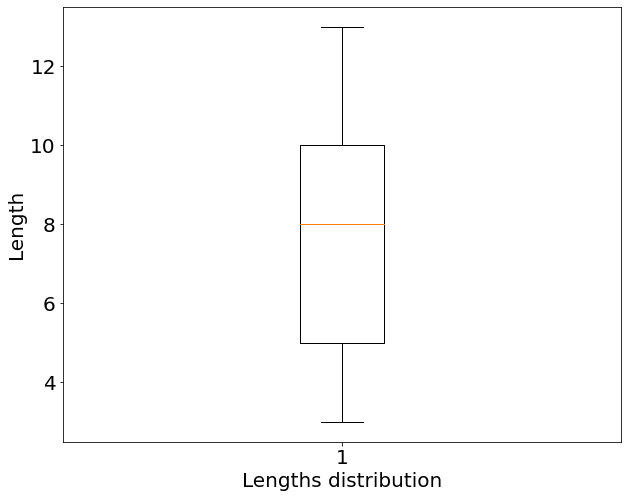
\includegraphics[width=0.35\textwidth]{/Users/carmenarmenti/Desktop/Thesis document/images/boxplot-length.png}
        \caption{\label{fig:CSdistribution}Code summarization task: data distribution.}
    \end{center}
\end{figure}
%%%%%%%%%%%%%%%%%%%%%%%
% TODO: Insert data distribution figure
%%%%%%%%%%%%%%%%%%%%%%%
Accordingly to the training set, the evaluation set was splitted in 4 sub-datasets as well, because the model trained on a defined level (or levels) of difficulty
needs to be evaluated on instances with the same complexity, according to the curriculum learning idea.\newline

\noindent\textbf{Training Scheduler.} Similarly to what happens in bug-fixing task, the training scheduler decides to sample from more harder data only when the model converges on the 
previous easier bucket. The convergence is assessed after a fixed number of epochs, after which early stopping with patience of 5 epochs
is run. Once the model converges on the first bucket, the training proceeds on the second and so forth. 

\subsection{Log generation task}
Inserting log messages is a practice broadly used and decide where to inject log statements, what information to report through it, 
and at which log level is as hard as it is crucial \cite{Mastropaolo2022}. In the following section Curriculum Learning approach 
is applied at log generation task. The dataset for this task is composed by couple of methods, where the source is the method without the log statement,
the target instead has not only the log statement but also the log message.\\
Those couples where used to train the model to generate and inject log statements in Java code.
If the training set for the training on the baseline model was composed by 106.382, the training set for the experiment with curriculum learning 
is of 105.985 instances. This was because of the Difficulty Measurer we choose to use: according to the latter, 397 instances had a null difficulty, hence
were excluded from the set. The same happend in the case of the evaluation set, 13.197 instances were used instead of 13.260. 
The test set ??? \newline


%\noindent\begin{minipage}{.45\textwidth}
%\begin{lstlisting}[language=Java, caption={Method},label={lst:buggy1}, mathescape=true, breaklines=true]{Name}
%    public CsvDestination setPath ( final String path ) 
%    { if ( csvFile != null ) 
%    { throw new UnsupportedOperationException ( ""Changing the value of path after opening the destination is not allowed."" ) ; } 
%    if ( outputChannel != null ) 
%    { try 
%    { outputChannel . close ( ) ; 
%    outputChannel = null ; } 
%    catch ( final IOException e ) { } } 
%    this . path = path ; 
%    return this ; }
%\end{lstlisting}
%\end{minipage}\hfill
%\begin{minipage}{.45\textwidth}
%\begin{lstlisting}[language=Java, caption={Method + log statement},label={lst:fixed1}, mathescape=true, breaklines=true]{Name}
%    public CsvDestination setPath ( final String path ) 
%    { if ( csvFile != null ) 
%    { throw new UnsupportedOperationException ( ""Changing the value of path after opening the destination is not allowed."" ) ; } 
%    if ( outputChannel != null ) 
%    { try 
%    { outputChannel . close ( ) ; 
%    outputChannel = null ; } 
%    catch ( final IOException e ) 
%    { log . error ( String . format ( ""Could not close file channel with CSV results for file %s."" , csvFile ) , e ) ; } } 
%    this . path = path ; 
%    return this ; }
%\end{lstlisting}
%\end{minipage}

%%%%%%%%%%%%%%%%%%%%%%%
% TODO: Insert instance ex.
%%%%%%%%%%%%%%%%%%%%%%%

\noindent\textbf{Difficulty Measurer.} Given the dataset at our dispose we choose as difficulty measurer the 
complexity of the instruction set in program execution tasks. More specifically we 
computed \textbf{cyclomatic complexity} through Lizard tool \cite{lizard}. Cyclomatic complexity
is a quantitative software metric developed by Thomas J. McCabe in 1976, used to indicate
the complexity of a program.  
It measures the number of linearly-independent paths through a program module. 
The measure is computed using the control-flow graph of the program where
the nodes of the graph correspond to sets of commands of a program, and
a directed edge connects 2 nodes if the second command might be executed
immediately after the first command. It can be applied to individual functions,
modules, methods or classes within a program. We decided to compute it on each of
the source methods.\\
It must be said that from the initial dataset were removed 397 instances whose
cyclomatic complexity was 0. Decided and computed the difficulty measure
for each instance, the dataset was ready to be used by the training scheduler.\newline

%%%%%%%%%%%%%%%%%%%%%%%
% TODO: Insert data distribution figure
%%%%%%%%%%%%%%%%%%%%%%%

\noindent\textbf{Training Scheduler.} Once again we observed the data distribution and considered the 3 quartiles
to divide the whole dataset in 4 subsets. Each of those represented a different level of difficulty.\\
As soon as the model converged on the current bucket, BLEU values after each epoch were assessed,
and early stopping was applied. We took the best model before divergence to restart the training 
from the following bucket. 


%%%%%%%%%%%%%%%%%%%%%%%
%RANDOM NOTES: 
%to use to sort the instances at dispose
%Only after this choice the initial dataset
%was divided in multiple smaller datasets For the task at issue here 
%the instances of th

%Once defined the measure, we were able to divide the initial dataset in smaller datasets so as to define 
%an incremental difficulty criteria to feed the model with. 

%For each of the task considered, a different metric to split the datasets was used.
%%%%%%%%%%%%%%%%%%%%%%%





 \chapter{Analysis of results}
In the following section the results 
achieved by NMT Encoder-Decoder with curriculum learning and
by the baselines for the three tasks we considered are reported.
We used different metrics for each of the tasks, depending on the metric used in the works
that introduced the baseline models.

\section{Bug fixing task}
To begin with, as assessed by Tufano \textit{et al.} \cite{Tufano2019} we used 
perfect predictions as a metric to evaluate the model performances. In the paper we took as reference
to test curriculum learning on, the authors differentiated 2 types of datasets; (i) the first one constituted by methods
whose length was up to 50 tokens and (ii) methods with length between 50 and 100 tokens. 
However, as stated in the previous sections
we considered the merge of the two datasets, 
therefore firstly we reproduced the canonical learning with the merged dataset and then we tested curriculum learning
approach.
Table~\ref{table:pp_bugfixing} reports the percentage %and numbers (?)
of bug fixing pairs correctly predicted
by the models for different beam sizes.
\begin{table}[h!]
    \centering
    \begin{tabular}{l|r|r}
    BEAM & Baseline & Baby-step\\ [0.5ex]
    \hline 
    1 & 5.22 \% & 5.34 \%\\ 
    5 & 13.00 \% & 19.41 \%\\
    10 & 16.55 \% & 25.16 \%\\
    15 & 18.38 \% & 28.64 \%\\
    20 & 19.60 \% & 30.84 \%\\
    25 & 20.51 \% & 32.39 \%\\
    30 & 21.29 \% & 33.69 \%\\
    35 & 21.93 \% & 34.93 \%\\
    40 & 22.26 \% & 35.72 \%\\
    45 & 22.73 \% & 36.47 \%\\
    50 & 23.02 \% & 37.39 \%\\ [1ex]
    \end{tabular}
    \caption{Models' performances}
    \label{table:pp_bugfixing}
\end{table}
Increasing the beam size, and generating more candidate patches accordingly,
the percentages of BFPs for which the models can perfectly generate the corresponding
fixed code - starting from the input buggy code - increases. If the baseline model can predict
the fixed code of 5.22\% of the BFPs with only one attempt, the same model together with 
curriculum learning approach performs predicting 5.34\% of the same BFPs. It is a 
better result,
but looking at bigger beam sizes, the model with curriculum learning performs 
even better, almost triplicating the percentage of perfect predictions of beam size 1 when 5 patches are generated,
reaching 37.39\% when 50 candidate patches are considered. Overall, it can be seen that
the improvement margin is constant.\\
On a second evaluation, we carried on a complementary analysis based on perfect predictions
obtained when the model generated 10 candidate patches for each prediction. 
As can be seen 
in Table~\ref{table:pp_bugfixing_overlap}, the combination between the two models 
leads to a reasonable percentage of perfect predictions, i.e. 42.38\%. However, the model 
with curriculum learning approach performs even better and on its own. Indeed, 44.63\% of BFPs are correctly predicted
only by the model with baby-step. On the other hand, only 12.97\% of perfect predictions are from the baseline.
\begin{table}[h!]
    \centering
    \begin{tabular}{l|r|r|r}
    \(Dataset (d)\) & \(Shared_d\) & \(OnlyBL_d\) & \(OnlyCL_d\)\\ [0.5ex]
    \hline 
    \(BF_{all}\) & 42.38 \% & 12.97 \% & 44.63 \%\\  [1ex]
    \end{tabular}
    \caption{Overlapping metrics: baseline and curriculum learning models.}
    \label{table:pp_bugfixing_overlap}
\end{table}
This result not only indicates that the two approaches are complementary for
the bug-fixing task, but also that the model with curriculum learning reports even 
better outcomes. Considering that the curriculum approach implemented is one of the easiest one,
those results recall the need to better tuning the approach with the aim of 
other improvements in the ability of such a model to exploit the knowledge acquired on 
this specific task. 

\section{Code summarization task}
In the study took as reference, the authors used different neural networks to 
assess the quality of their work. So, the comparison between our results and theirs
is not really straigh-forward. However, as said before, we reproduced the experiment on a baseline model,
i.e. on the model without any curriculum learning approach applied.
The experiment on the baseline model totalized a BLEU-A score of 13.70 that is way lower than 
each of the scores obtained by the authors of LeClair \cite{Leclair2020}. 
\begin{table}[h!]
    \centering
    \begin{tabular}{l|r|r|r|r|r}
     & BLEU-A & BLEU-1 & BLEU-2 & BLEU-3 & BLEU-4\\ [0.5ex] 
     \hline
     Baseline & 13.70 & 38.8 & 18.4 & 10.6 & 7.1\\  
     Baby-step & 13.29 & 38.0 & 17.8 & 10.2 & 7.0\\ [1ex]
     \end{tabular}
    \caption{BLEU values summary .}
    \label{table:1}
    \end{table}
On the other hand, the BLEU value after the experiment on the model together with the curriculum approach
scored a value of 13.29, which is lower than the results achieved by the baseline, then lower than the BLEU values in \cite{Leclair2020}.
This means that in this case the curriculum approach does not work in the view of collecting better results.
However, it must be said that the model used in our experiment is different from the 
model used by the authors of the paper we took as reference; this might mean that the differences observed
may be caused by the fact that the original model should have been used and not on the technique applied.\\
Also on perfect predictions we do not have better results, and we can observe - as showed in Table~\ref{table:2} - that the values are not 
that much distant one from another.
\begin{table}[h!]
    \centering
    \begin{tabular}{l|r|r} 
    %\multicolumn{3}{c}{Perfect predictions} \\
    & Baseline & Baby-step\\ [0.5ex] 
    \hline
    BEAM 1 & 4.66 \% & 4.64 \%\\  
    BEAM 5 & 6.68 \% & 6.53 \% \\ 
    BEAM 10 & 7.75 \% & 7.52 \%\\
    BEAM 15 & 8.36 \% & 8.07 \%\\
    BEAM 20 & 8.84 \% & 8.51 \%\\
    BEAM 25 & 9.17 \% & 8.83 \%\\
    BEAM 30 & 9.47 \% & 9.06 \%\\
    BEAM 35 & 9.74 \% & 9.29 \%\\
    BEAM 40 & 9.90 \% & 9.49 \%\\
    BEAM 45 & 10.06 \%& 9.67\%\\
    BEAM 50 & 10.24 \%& 9.83\%\\ [1ex]
    \end{tabular}
    \caption{Perfect predictions summary.}
    \label{table:2}
\end{table}
\section{Log generation task}
 \chapter{Conclusion}
In this work we wanted to test the curriculum learning approach on code related tasks.
In order to test this new technique we decided to take as reference two important papers and to compare 
our findings to the results achieved only by using deep learning models.
As explained in Chapter \ref{chapter:MAO} there are well-known advantages that curriculum learning
brougth to the current state of the art. However, it is also true that advantages and benefits depend highly on the data 
the model takes in input and consequently the results with curriculum applied might not always be better than 
those obtained on the plain model. 
In fact, we could notice that if on bug-fixing task the model with curriculum learning 
took better results not only in terms of performance but also of accuracy, 
in the case of the second task, i.e. code summarization, the results achieved in \cite{Leclair2020}
are definetly better.
Nevertheless, it must be said that we focused our attention on the technique used to train, but in order to achieve better 
results other changes at the baseline model migh be done. To illustrate, if for the first task we used the very same model 
to train both the baseline and the curriculum learning approach, in the second case the model used as for the training was not the 
one used by the authors in \cite{Leclair2020}. The negative results achieved might indicate differen scenarios. One possible reason might be that 
the approach used is not suitable for code-summarization-like tasks, since it is the case of a NLP objective to learn for the model.
A more robust technique might bring positive results.
Moreover, those negative results might not be that negative. We proposed an approach that worked very well on a task that was originally tested on the same 
training model. It was not the case for the second one. Reproducing the experiment on the same model used by LeClair \cite{Leclair2020} may possibly bring different results.
If that was the case, the curriculum learning would be an approach suitable for any deep learning model.
To sum up, by experimenting two tasks and collecting one positve and one negative result we can acknowledge that curriculum learning 
outcomes highly depend on the training data and the approach must be settled differently for each task.


 \begin{acknowledgements}

\addchaptertocentry{\acknowledgementname}
Five years ago, when I decided to start studying to be part of the IT industry someday, 
I had no idea what was waiting for me. 
I did not get into computer science before starting university, and because of that 
I wanted to ask Prof. Rocco Oliveto - which at that time already was the chair of the bachelor program - for his advice 
in this regard. Even though I did not know why, on talking to him I immediately felt the path I was about to choose was right for me. 
I trusted him and I trusted my instincts. \\
Today, after five years - one of which I studied abroad - I think my place in the world is starting to become clear.
Never have I ever felt more confident on the decision I made. Yet I am a person who more often than needed struggles with self-confidence.\\
\newline
I owe Prof. Rocco Oliveto - my advisor and one of the most inspiring teachers I have encountered
in my course of study - a huge thank you, for everything mentioned above and more. Not only was he the reason why I started my journey in one of the most impactful and topic-broad field, 
but he also gave me a lot of opportunities to grow educationally and personally trough both his academic lectures and life-lessons.
Thank you for supporting me during the last few years and for being part of the professional future I have just started to create.

I would also like to thank Prof. Rocco Oliveto, Prof. Gabriele Bavota, and all the UNIMOL and USI staff who gave me the life-changing opportunity to 
achieve the double degree. 
Spending the last year of my Masters at Università della Svizzera Italiana, was pivotal. Even though it was
really tough, it came at a moment in my life when I needed it. 
Getting through that extremely challenging and demanding 
time was genuinely essential in teaching to me what really matters, not only career-wise, but also in life. Thank you 
for the unique opportunity you gave me, and your wholehearted support.

I thank Prof. Gabriele Bavota who since the very first moment I met him, made himself available for any kind of support. 
Thank you for not missing any opportunity to remind me that there was someone on the other side who believed in me. Also, thank you 
for giving me the chance to work on the master thesis with your advice. I have learned so much.

This piece of work would not have been possible without the help of Antonio Mastropaolo. 
Thank you for all your time and your words of advice, I will not foget them.\\
\newline
I owe a huge thank you to Tania Clarke. Not only is she the best English teacher I have ever had, 
but for the past two years she has been a very important figure for me. A source of knowledge
of a language that I have always wanted to perfect and learn more about. Thank you for always being supportive.
Studying aside, your letting me talk and your simple and direct advice helped me.\\
\newline
There are no words to thank my family, source of unconditional love and endless support. 
The only thing in the whole world which I cannot live without;
the source of strength, courage, foresight, wisdom; the reason why I am who I am.
Thank you mom and dad for giving me the right discipline; thanks for being my pillars, 
empathic objectivity on one side and hopeful rationality on the other. Thank you Ugo and Vito, 
brothers as annoying as they are attentive and loving. Thank you for always being by my side. What would I do without you?\\
\newline
My abroad experience would have not been the same if I had not met Ottavio, Daniel, Gianlorenzo, Federico, and Isabella. 
Thanks for all the sharing views we talked about, the fun we had together, and the memories we collected. I feel very grateful to have met you.
You now take up a part of my heart.\\
\newline
Special thanks go to Martina, Antonio, and Silvia. 
You could see how I really am and I truly feel extremely grateful 
for standing there for me, and not only when I really needed it. 
I will never forget your constant support, that has emerged a little more in the past year, but that was 
just a testament to a solid and sincere frienship. I am glad of having you on my side and I will always be by yours.
You can count on it!\\
\newline
Thank you all.
\end{acknowledgements}

%\appendix
%\chapter{Appendix}


%%%%%%%%%%%%%%%%%%%%%%%%%%%%%%%%%%%%%%%%%%%%%%%%%%%%%%%%%%%%%%%%%
%%%	BIBLIOGRAPHY %%%%%%%%%%%%%%%%%%%%%%%%%%%%%%%%%%%%%%%%%%%%%%%%
%%%%%%%%%%%%%%%%%%%%%%%%%%%%%%%%%%%%%%%%%%%%%%%%%%%%%%%%%%%%%%%%%

\newpage
\bibliographystyle{abbrv}
% \bibliographystyle{plainnat}
\bibliography{biblio}

\end{document}



